\section{Project Schedule}
Below is the Gantt chart of our project Schedule to perfrom these specific tasks between these time frames.
\begin{figure}[H]
    \centering
        \includegraphics[width=400px]{Diagrams/Gantt_Chart.png}
    \caption{Gantt Chart of Schedule}
\end{figure}

\lstset{frame=tb,
  language=PHP,
  aboveskip=3mm,
  belowskip=3mm,
  showstringspaces=false,
  columns=flexible,
  basicstyle={\small\ttfamily},
  numbers=none,
  numberstyle=\tiny\color{gray},
  keywordstyle=\color{blue},
  commentstyle=\color{dkgreen},
  stringstyle=\color{mauve},
  breaklines=true,
  breakatwhitespace=true,
  tabsize=3
}
\section{Setup Guide to run Code Connect Locally}
\begin{enumerate}
    \item \textbf{Prerequisite:}
    \begin{enumerate}
        \item XAMPP
        \item Operating System that support XAMPP.
        \item Internet Connection for CDN libraries.
        \item Project Files Cloned from Git Hub.
    \end{enumerate}
    \item Clone Repo in htdocs/\\
    \begin{verbatim}
git clone https://github.com/sushantbramhacharya/CodeConnectBE.git
    \end{verbatim}
    \item Open PhpMyAdmin by going into \url{http://localhost/phpmyadmin}
    \item Create Database codeconnect
    \item Import Database codeconnect.sql from folder cloned using Import button located in navbar.
    \item Open XAMPP Control Panel.
    \item Start Apache and MySQL Servers.
    \item Run it on http://localhost/ or codeConnect directory.
\end{enumerate}
\section{Running Hosted Code Connect}
\begin{enumerate}
    \item Open Mobile/Desktop Browser .
    \item Go to \url{https://sushantbramhacharya.com.np/codeconnect}.
\end{enumerate}
\section{MySQL Connection in our CodeConnect PHP}
\vspace{1cm}
\begin{lstlisting}
    <?php
    $servername = "localhost";
    $username = "root";
    $password = "";
    $dbname = "codeconnect";

    $conn = new mysqli($servername, $username, $password, $dbname);

    if ($conn->connect_error) {
        die("Connection failed: " . $conn->connect_error);
    }
    ?>
    \end{lstlisting}
    \newpage
\section{JQuery AJAX Used in CodeConnect}
\vspace{1cm}
\begin{lstlisting}
    $.ajax({
    url: 'url',
    method: 'GET',
    data: { key1: 'value1', key2: 'value2' },
    dataType: 'json',
    success: function(response) {
        console.log(response);
    },
    error: function(xhr, status, error) {
        console.log('Error: ' + error);
    }
    });

    \end{lstlisting}
    \section{Database Screenshots}
    Here the Screenshots of tables used in database of code connect.
    \begin{figure}[H]
        \centering
            \includegraphics[width=420px]{db_img/user.png}
        \caption{User Table}
    \end{figure}
    \begin{figure}[H]
        \centering
            \includegraphics[width=150px]{db_img/certifications.png}
        \caption{Certifications Table}
    \end{figure}
    \begin{figure}[H]
        \centering
            \includegraphics[width=200px]{db_img/connections.png}
        \caption{Connections Table}
    \end{figure}
    
    \begin{figure}[H]
        \centering
            \includegraphics[width=400px]{db_img/discussion.png}
        \caption{Discussion Table}
    \end{figure}
    
    \begin{figure}[H]
        \centering
            \includegraphics[width=170px]{db_img/geek.png}
        \caption{Geek Table}
    \end{figure}
    
    \begin{figure}[H]
        \centering
            \includegraphics[width=200px]{db_img/messages.png}
        \caption{Messages Table}
    \end{figure}
    
    \begin{figure}[H]
        \centering
            \includegraphics[width=400px]{db_img/projects.png}
        \caption{Projects Table}
    \end{figure}
    
    \begin{figure}[H]
        \centering
            \includegraphics[width=150px]{db_img/saved.png}
        \caption{Saved Table}
    \end{figure}
    
    \begin{figure}[H]
        \centering
            \includegraphics[width=220px]{db_img/skills.png}
        \caption{Skills Table}
    \end{figure}
    
    \begin{figure}[H]
        \centering
            \includegraphics[width=200px]{db_img/comments.png}
        \caption{Comments Table}
    \end{figure}
\section{Supervisor Consultation Form}
\begin{figure}[H]
    \centering
    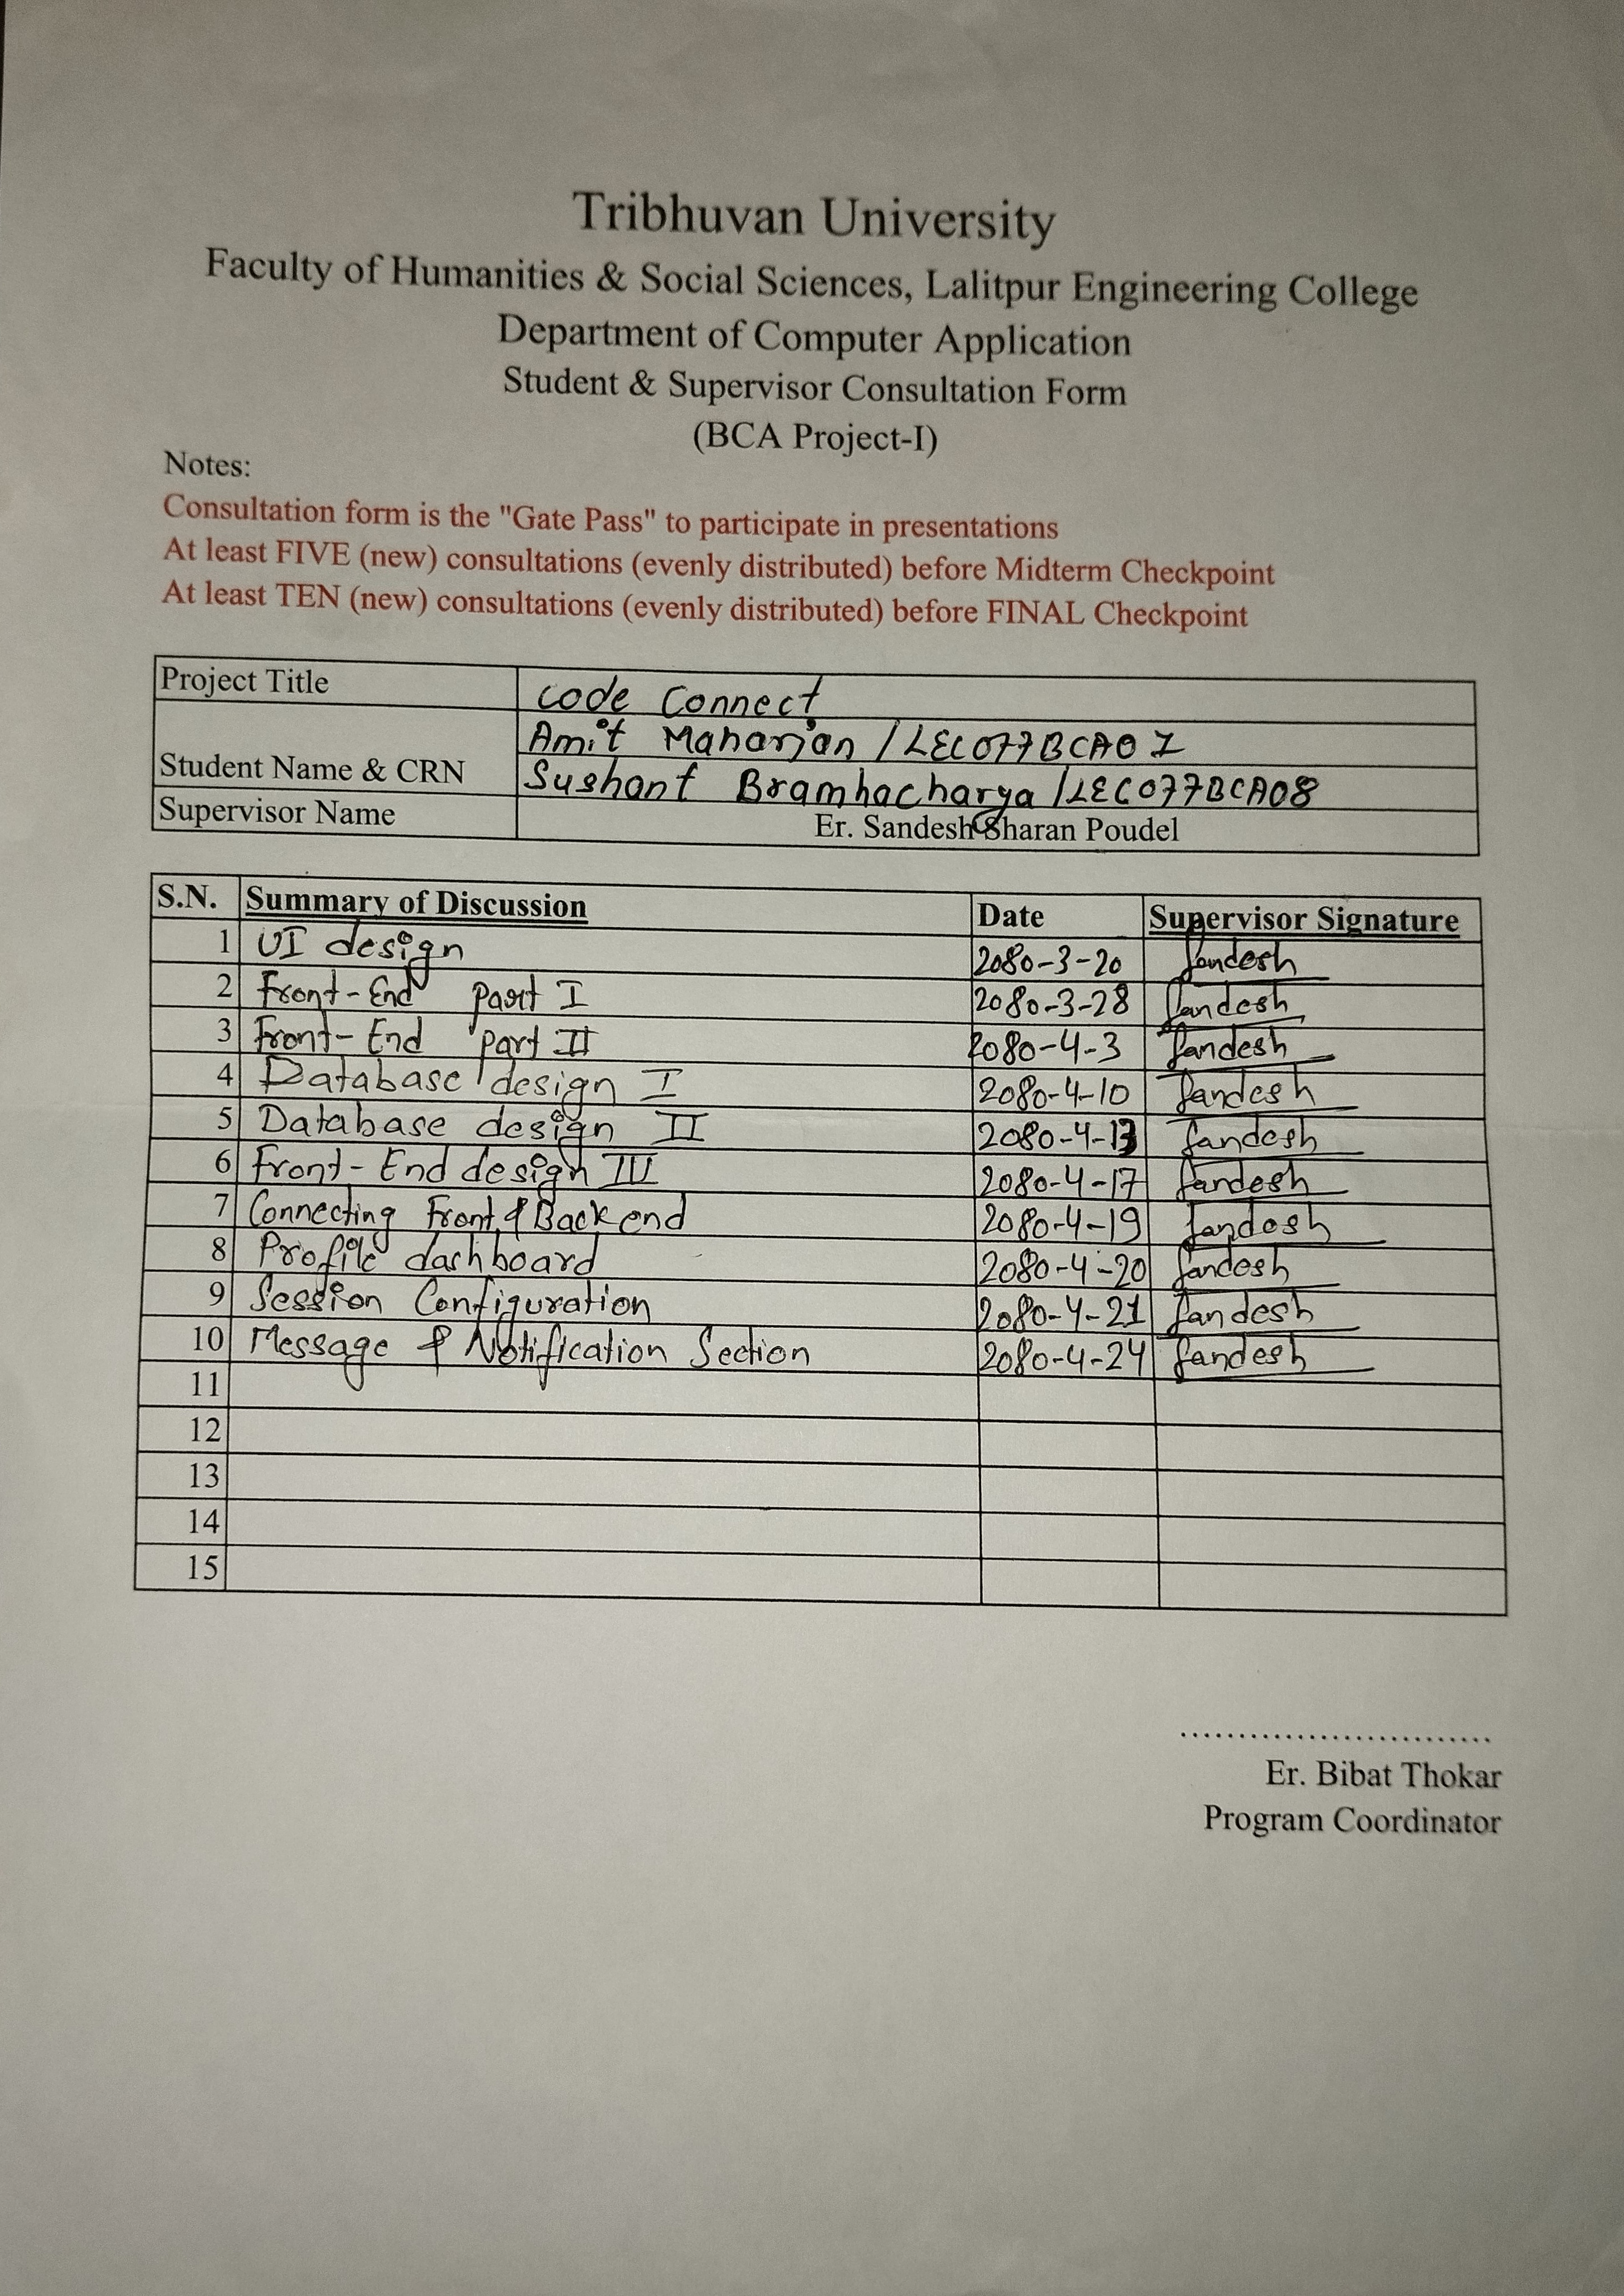
\includegraphics[width=400px]{Appendix/supervisor-form.jpg}
    \caption{Supervisor Consultation Form}
\end{figure}


